% TODO klar benennen, dass wir uns jetzt ein Fallbeispiel Anschauen

\SetNextBackground{\includegraphics[width=\paperwidth,page=3]{hpke-slide-designs}}
\begin{frame}{Die vier Domänen der Sicherheit sind…}
  % GOAL Orientierung, wo wie gerade hinschauen für das Fallbeispiel
%  \Large
%  \begin{columns}[c]
%    \begin{column}{.5\linewidth}
%      \textbf{Luftfahrt}
%    \end{column}
%    \begin{column}{.5\linewidth}
%      Automobile
%    \end{column}
%  \end{columns}
%  \vfill
%  \begin{columns}[c]
%    \begin{column}{.5\linewidth}
%      Medizintechnik
%    \end{column}
%    \begin{column}{.5\linewidth}
%      Automatisierung
%    \end{column}
%  \end{columns}
\end{frame}

\interlude[1]{Kryptografie in der Avionik}


\SetNextBackground{\includegraphics[width=\paperwidth,page=4]{hpke-slide-designs}}
\begin{frame}[c]{Sichere Kryptografie in der Avionik}
%  % GOAL Aufzeigen, das (gute) Cryptography in Avionik fehlt
%  \vspace{4em}
%  \footnotesize
%  (Gähnende Leere)
\end{frame}

\SetNextBackground{\includegraphics[width=\paperwidth,page=5]{hpke-slide-designs}}
\begin{frame}[c]{Zum Erschrecken aller…}
  % GOAL Aufzeigen, dass auch fortschrittliche Planung durch Mangelnde Kryptoagilität zum scheitern verurteilt ist (LDACS Paper)
  \begin{columns}[fullwidth,c]
    \begin{column}{.5\linewidth}
%      \begin{itemize}

        \footnotesize
        …wird in der Luftfahrt heutzutage keine sichere Kryptografie eingesetzt. 
%      \end{itemize}
    \end{column}%
    \hfill
%    \begin{column}{.5\linewidth}
%      % GOAL Digital Drahtlos Kommunikation seit 45 jahren
%      % GOAL Erste ernste zunehmende Kryptographie in 2007 eingeführt, aber quasi keine Verbreitung
%      % GOAL 2021 dann der erste Vorschlag, für einen hybridig post-quaten sicheren Datalink...
%      % GOAL ... aber noch vor dem Rollout und nach nur einem Jahr ist die chiffre gebrochen :(
%      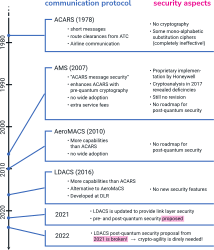
\includegraphics[width=.92\linewidth]{graphics/history of cryptography in avionics}
%    \end{column}
  \end{columns}
\end{frame}


\SetNextBackground{\includegraphics[width=\paperwidth,page=6]{hpke-slide-designs}}
\begin{frame}[c]{Kryptographie in der Avionik: Unser Ansatz}
  % GOAL HPKE ist ein standard  mit festen interface, dennoch sind die internen Primitive modular
  \begin{columns}[fullwidth,c]
    \begin{column}{.65\linewidth}
      \begin{itemize}
        \item Kryptographischer Standard:\\
        Hybridge Public Key Encryption (HPKE)
        \item Schnittstelle aus HPKE
        \begin{itemize}
          \item Seal: Nachricht verschlüsseln (und signieren)
          \item Open: Nachricht entschlüsseln (und prüfen)
        \end{itemize}
      \end{itemize}
    \end{column}%
    \hfill
  \end{columns}
\end{frame}


\SetNextBackground{\includegraphics[width=\paperwidth,page=8]{hpke-slide-designs}}
\begin{frame}[c]{Flexible Einsatzszenarien, gleiche Schnittstelle}
  % GOAL Auswahl der Primitive erlaubt tradeoffs, Schnittstelle bleibt gleich
  \begin{columns}[fullwidth,c]
  \hfill
    \begin{column}{.35\linewidth}
      \begin{itemize}
        \item Pre oder post-Quantum?
        \item Mehr oder weniger Speicherbedarf?
        \item Schnell oder langsam?
        \item Post-quantum Authentisierung? 
      \end{itemize}
    \end{column}%
%    \begin{column}{.65\linewidth}
%      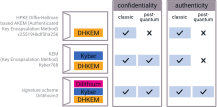
\includegraphics[width=\linewidth]{graphics/hpke variants}
%    \end{column}
  \end{columns}
\end{frame}


\SetNextBackground{\includegraphics[width=\paperwidth,page=9]{hpke-slide-designs}}
\begin{frame}[c]{Partitionen zur Integration in die Avionik}
%  \centering 
%  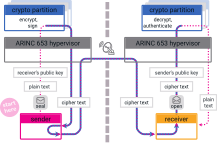
\includegraphics[width=0.8\linewidth]{graphics/crypto partition}
\end{frame}

% GOAL Aufzeigen, dass und wie Modularität der Schlüssel für Kryptoagilität in der Safety ist
% GOAL Aufzeigen, dass Integration einfach möglich, und zulassungsfreundlich gemacht werden kann


% TODO eine folie über Benchmarks?


% \begin{frame}[c]{Ansätze für Verbesserung in beiden Bereichen}
%   % GOAL ist mir unklar
%   % TODO wucke refine 

%   Verifikationstechniken
%   \vspace{0.5em}

%   {\footnotesize Zertifizierung <-> Sicherheitsbeweise}
%   \vspace{1.5em}
%   % Formaler Beweis kann Teil der Evidence für Zertifizierung sein
%   % Annahmen und Anforderungen müssen in den Zertifizierungsdokumenten festgehalten werden
%   % Evidence = Belege, warum Annahmen wahr sind oder Anforderungen erfüllt sind
%   % Unabhängigkeit zwischen Implementierer und Verifizierer
%   % 
%   % - Wanja
%   %
%   % Agreed; geht mir eher darum die generelle Vorgehensweise zu beschreiben als formell korrekt jede Möglichkeit durchzugehen.
%   % Ist beweisführung in der Avionik denn üblich?
%   % 
%   % – Karolin

%   Kompartmentalisierung
%   \vspace{0.5em}

%   {\footnotesize Partitionierung <-> Brokerarchitekturen}
%   \vspace{1.5em}
%   % Aufteilung erleichtert sukzessive Absicherung einzelner Komponent
%   % Gleichzeitig: Faultcontainment
%   % Modularisierung macht updates einfacher, da klare interfaces zwischen Modulen

%   % Diagram Idee: Konfidenzarchitektur
%   %
%   % 1. Identifiziere mögliche Fehlerursachen
%   % 2. Ist ein Fehler relevant?
%   %   - Falls Nein, warum nicht? Evidence!
%   % 3. Welche Effekte hat der Fehler?
%   % 4. Wie kann der Fehler verhindert/eingedämmt/mitigiert werden?
%   % 5. Wie kann der Fehler erkannt werden?
%   % 6. Validiere Annahmen von 3. - 5.
%   % 7. Review durch unabhängigen Assesor
%   %
%   % -- wucke13
%   %
%   % Passt das denn in das Gegenüberstellungsscheme? Also wie bringen wir den Vergleich Avionik vs Crypto rein.
%   %
%   % -- karolin

%   => Kryptoagilität
% \end{frame}
